\chapter{Pyramid Matching Score for Detection}
\label{chp5}

\section{Introduction}

The results of chapter \ref{chp4} is promising on the two experimental datasets, however, the efficiency is not good. Besides, theories which explain Hough transform-based methods are not satisfactory. In this chapter, a detection method is proposed. It will fill up the gap between theory and practise for Hough transform, work efficiently, and make use of the mutual information encoded in image features of the same object.

Detection methods still mainly follow the sliding-window schema or have similar structure with Hough transforms. While the focus of the later is to infer about object status by use each online feature as query against a well-trained codebook. These methods fail to consider target objects as a whole at the beginning. The problem of sliding-window is that it often ignores positional information when also following bag of features~\cite{bgf}. In the method of \cite{spmk}, positional information is considered in the kernel function. Here the kernel function\cite{kmts} is used in classifiers, which are usually support vector machines.

The method proposed here consider object as a whole during detection. 


This Chapter is organized as follows. Section \ref{rw5} reviews most related work. Section \ref{dt5} propose the training and detecting procedure. Section \ref{exp5} gives experimental results. Section \ref{conc5} concludes this chapter.

\section{Related Work}
\label{rw5}
The bag-of-feature~\cite{bgf} schema successfully improves detection performance, while still there are information which are left behind in images. The positional information is not fully made use of, even the method of \cite{kmts}. While \cite{uspl} provides a method to model the relationship between object parts, there are two many parameters to estimate in their model, which requires large amount of training data for acceptable performance.

In the method proposed in ~\cite{ac222}, each object is modeled as a graph, when match each object with another, constrains are made not only between the two objects, but also between different features of the same object. The relationship between elements of the same object is important. However, the inefficiency of this method prevents it from directly being used for object detection, while its performance on matching the same object under different views is promising.

The method in \cite{lbt1} instead of building some parametric or non-parametric model, directly maps the labels of similar images in the training images to the current image. In this manner, the descriptive ability of model can be left alone, which in return makes the method robust. However, this kind of methods heavily rely on the manually marked labels in the training dataset, while such labels are very expensive in human power and computation.

The pyramid matching score method is most related to methods using \cite{pmk} or \cite{kmts} as kernel functions, methods employ Hough transforms, and also the methods proposing efficient solution space searching techniques~\cite{bab}.





\subsection{Pyramid Matching}

The Pyramid Matching method is designed to find the best one-one matching between two point(feature) sets in a heuristic manner.

Given two point sets, ${S_1} = \{ {u_1},{u_2},...,{u_m}\} $
 and ${S_2} = \{ {v_1},{v_2},...,{v_n}\} $
, there exists a best one-one matching ${\pi}^*$ that minimizes the sum of $L1$
-distances between matched pairs,

\[
{\pi ^*} = \arg \mathop {\min }\limits_\pi  \sum\limits_{{u_i} \in {S_1}} {||{u_i} - {v_{\pi (i)}}|{|_1}} \ .
\]
Here $m<n$, and $\pi$ maps each feature $u_i$ in $S_1$ to a unique feature ${{v_{\pi (i)}}}
$ in $S_2$.

The best matching exists, and can be found by simple brute-force methods. In special cases, the Hungarian algorithm is also applicable.

Sub-optimal solution can be found by heuristic methods. A very intuitionistic method is to find matched pairs of nearest distance, exclude corresponding points from both point sets, and repeat until no pair can be found.

The methods mentioned above are not efficient enough. The Pyramid Matching method is straightforward. Divide the space into very fine grids, and exclude all pairs of points, each of which exists in the same grid. Then divide the space into coarser grids, and continue to exclude matched pairs of points until no pair can be found.

However, in order to know the sum of distances between matched pairs, the distance between two matched points still needs to be calculated. In order to avoid such calculations, the "distance" is directly assigned by how fine the grids are when the two points are considered as matching.

The Pyramid Matching method is very efficient.

\subsection{Pyramid Matching Score}

The Pyramid Matching Score measures the confidence about one rectangle contains an object of a given type. One "point" set contains all the image features contained in the rectangle to be measured, the other "point" set is a "super template". The template is trained by inserting all features from training images.

When SIFT is used, PCA is used to do dimension reduction. And the position information of each feature can be used by adding them as two extra dimensions of the feature.

\section{Detection}
\label{dt5}

Sliding-window schema is employed to check with the defined Pyramid Matching Score on all sub-images of the test image for detection decisions.

\section{Experimental Results}
\label{exp5}


\begin{figure}
\centering

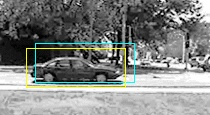
\includegraphics[scale=0.75]{test-0_good.jpg}
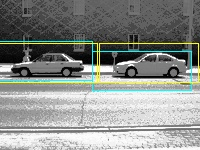
\includegraphics[scale=0.75]{test-10_good.jpg}
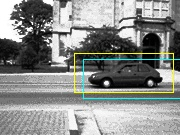
\includegraphics[scale=0.75]{test-14_good.jpg}
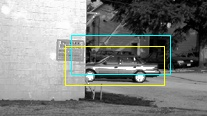
\includegraphics[scale=0.75]{test-16_good.jpg}
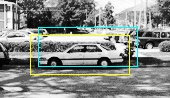
\includegraphics[scale=0.75]{test-20_good.jpg}
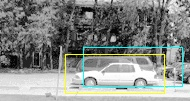
\includegraphics[scale=0.75]{test-21_good.jpg}
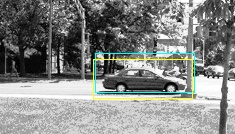
\includegraphics[scale=0.75]{test-22_good.jpg}
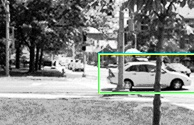
\includegraphics[scale=0.75]{test-24_good.jpg}
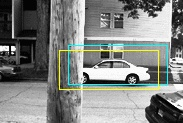
\includegraphics[scale=0.75]{test-29_good.jpg}
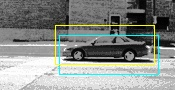
\includegraphics[scale=0.75]{test-2_good.jpg}
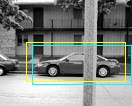
\includegraphics[scale=0.75]{test-31_good.jpg}
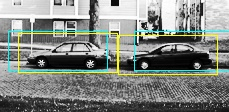
\includegraphics[scale=0.75]{test-3_good.jpg}
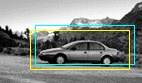
\includegraphics[scale=0.75]{test-5_good.jpg}
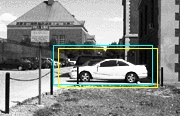
\includegraphics[scale=0.75]{test-8_good.jpg}


\caption[Detection Results on UIUC cars]{Detection results on UIUC cars~\cite{cds}. Yellow color marks ground truths, while blue marks detections.}
\label{fig:c5r}
\end{figure}

In Figure \ref{fig:c5r}, are some good results on UIUC cars. And new experiments will be added.
\begin{figure}
\centering

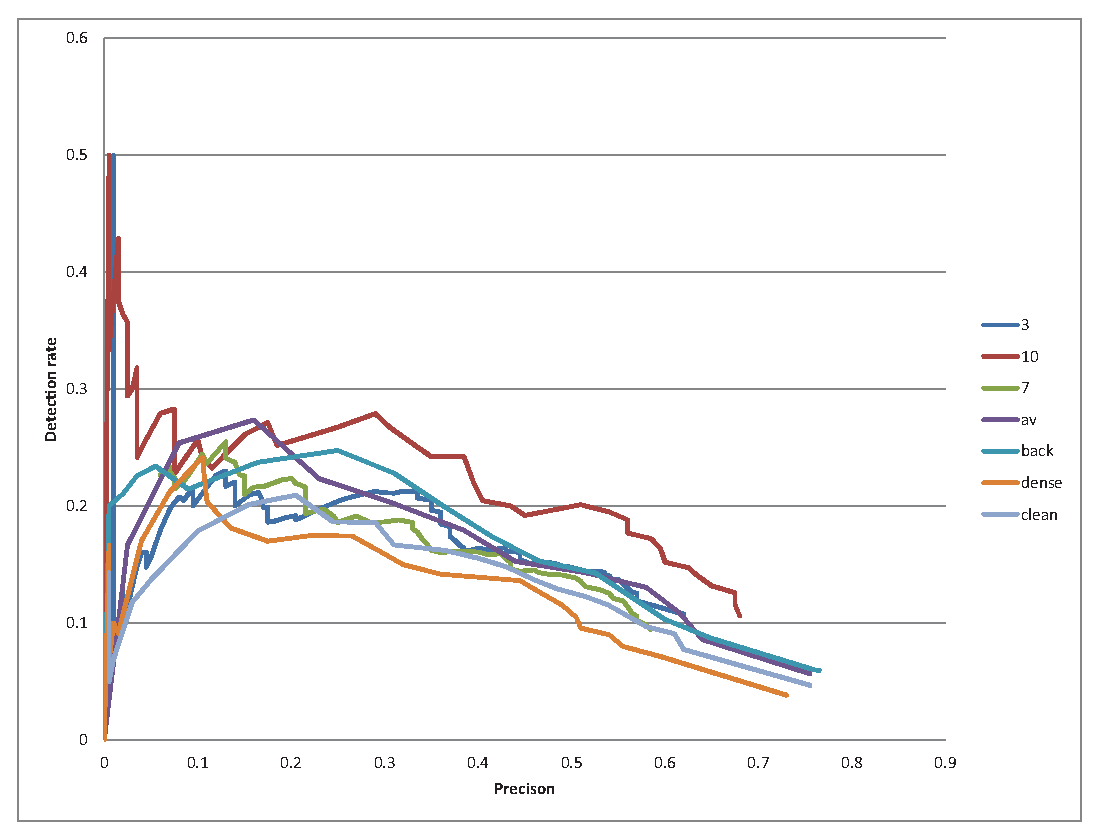
\includegraphics[width=1\textwidth,bb=0 0 480 425]{pms.eps}


\caption[Result evaluation]{Results evaluation on UIUC cars with different implementation parameters.}
\label{fig:c52}
\end{figure}

In Figure \ref{fig:c52}, evaluations are given.

\section{Chapter Conclusion}
\label{conc5}

There will be several experiments to be summarized for this chapter, and also several experiments to be added.
